\subsection{Related Work}
\label{subsect:related-work}

% https://dx.doi.org/10.7155/jgaa.00366
\begin{frame}
  \frametitle{\insertsubsection}
  \begin{itemize}
    \item \quoted{Drawing Graphs with Few Arcs} (2015) \begin{itemize}
      \item Lower and upper bounds of required entities
      \item Only very specific classes of graphs
    \end{itemize}
    \vspace{0.5cm}
    \centering
    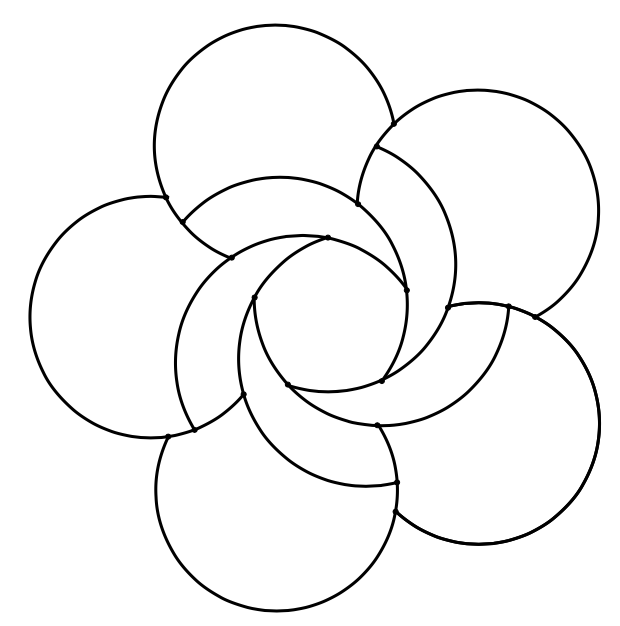
\includegraphics[height=4cm,natwidth=620,natheight=626]{Resources/Schulz.png}
  \end{itemize}
\end{frame}

% https://dx.doi.org/10.1007/978-3-642-25878-7_31
\begin{frame}
  \frametitle{\insertsubsection}
  \begin{itemize}
    \item \quoted{Force-directed Lombardi-style Graph Drawing} (2011) \begin{itemize}
      \item Attempt to improve angular resolution
      \item Soft constraint
    \end{itemize}
    \vspace{0.5cm}
    \centering
    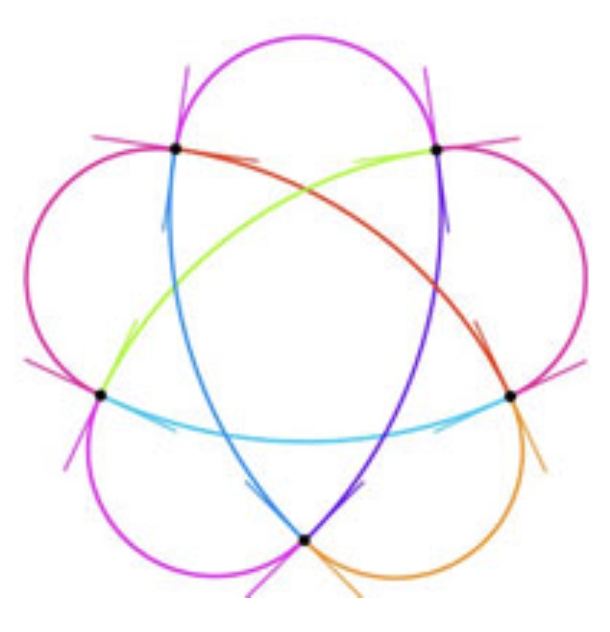
\includegraphics[height=4cm,natwidth=610,natheight=632]{Resources/Lombardi.png}
  \end{itemize}
\end{frame}

% https://dx.doi.org/10.1007/3-540-58950-3_391
\begin{frame}
  \frametitle{\insertsubsection}
  \begin{itemize}
    \item Magnetic-spring algorithm (1994) \begin{itemize}
      \item Attempt to align edges with a magnetic field
      \item Soft constraint
    \end{itemize}
    \vspace{0.5cm}
    \centering
    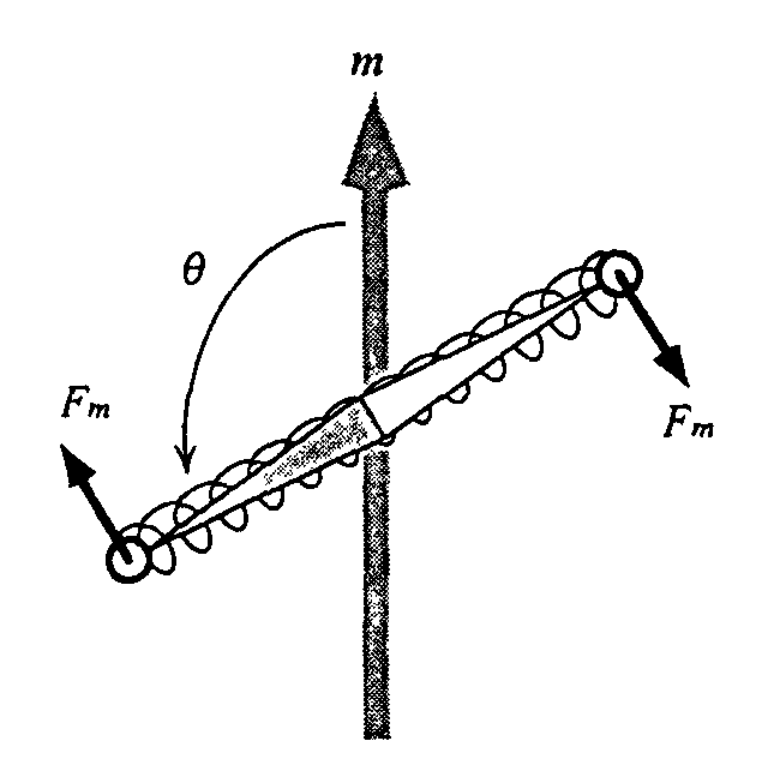
\includegraphics[height=4cm,natwidth=764,natheight=780]{Resources/MagneticSprings.png}
    \hspace{0.5cm}
    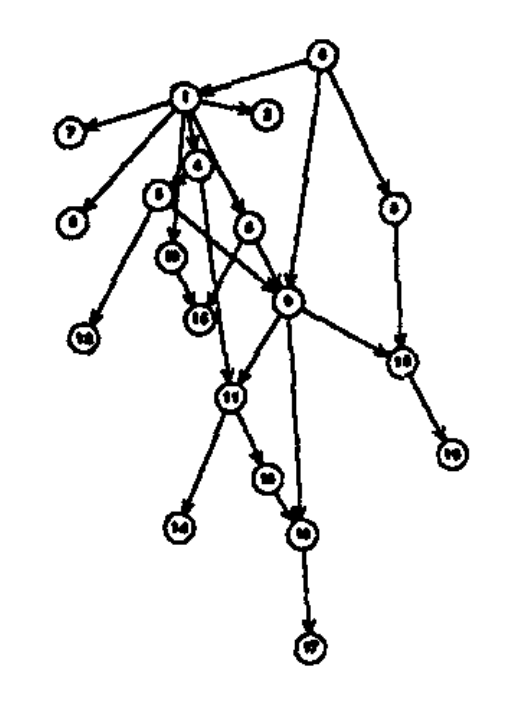
\includegraphics[height=4cm,natwidth=506,natheight=710]{Resources/MagneticDrawing.png}
  \end{itemize}
\end{frame}

% https://doi.org/10.1007/3-540-46648-7_36
\begin{frame}
  \frametitle{\insertsubsection}
  \begin{itemize}
    \item PrEd (1999) \begin{itemize}
      \item Preserves edge crossing properties
      \item Hard constraint
      \item Does not reduce the number of degrees of freedom
    \end{itemize}
    \vspace{0.5cm}
    \centering
    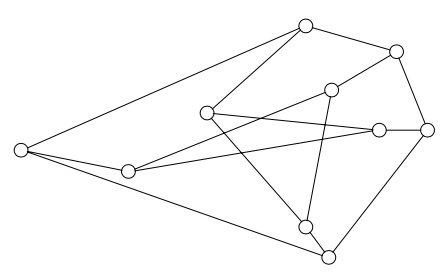
\includegraphics[height=2.5cm,natwidth=440,natheight=276]{Resources/PrEd-before.png}
    \hspace{0.5cm}
    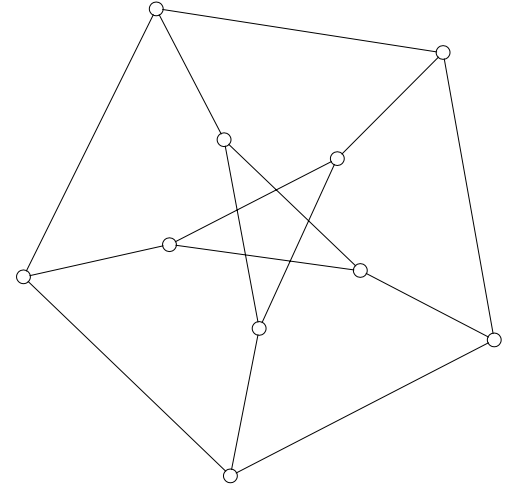
\includegraphics[height=4cm,natwidth=520,natheight=492]{Resources/PrEd-after.png}
  \end{itemize}
\end{frame}
